% ═══════════════════════════════════════════════════════════════════════════════
\chapter{Implementation}
% ═══════════════════════════════════════════════════════════════════════════════

\section{Introduction}

This chapter covers the technical implementation of the MES-X dependency
traceability system, describing how the proposed architecture was built into a
working full-stack application. The system brings together work items, pull
requests, commits, branches, tags, sprint planning data, and AI-assisted
review into a single coherent workflow.

The chapter starts with the technology stack, then walks through the
development approach, backend modules, frontend integration, deployment setup,
and the quality practices used to validate the final product.

% ──────────────────────────────────────────────────────────────────────────────
\section{Technology Stack and Architecture}

MES-X is built on a modern full-stack architecture designed to handle
large-scale dependency graph reconstruction and traceability analysis
efficiently.

\subsection{Web Application Layer (Frontend)}

The frontend is the main interface operators use to run and explore
traceability analyses. It is built for responsiveness and clarity when
rendering complex dependency graphs.

\textbf{Technical specifications:}
\begin{itemize}
  \item \textbf{Framework:} Vue 3 with TypeScript
  \item \textbf{UI framework:} Quasar component system
  \item \textbf{Build tool:} Vite
  \item \textbf{Purpose:} trace execution, progressive visualization, and dependency navigation
\end{itemize}

\begin{figure}[htbp]
  \centering
  
\includegraphics[width=0.45\linewidth]{img/logo/vuejs.png}
  \caption{Frontend technology used: Vue 3 for building the user interface}
  \label{fig:vue-logo}
\end{figure}

% ──────────────────────────────────────────────────────────────────────────────
\subsection{Backend Service Layer}

The backend is the core of the system. It handles traceability logic and
exposes structured APIs for both single and batch analysis.

\textbf{Technical specifications:}
\begin{itemize}
  \item \textbf{Framework:} NestJS (TypeScript)
  \item \textbf{API styles:} REST for queries, SSE for streaming
  \item \textbf{Role:} orchestrating dependency graph construction
\end{itemize}

The backend is organized into domain-driven services, each responsible for
processing and enriching a specific part of the traceability data.

\begin{figure}[htbp]
  \centering
  
\includegraphics[width=0.45\linewidth]{img/logo/nestjs.png}
  \caption{Backend technology used: NestJS for scalable server-side architecture}
  \label{fig:nestjs-logo}
\end{figure}

% ──────────────────────────────────────────────────────────────────────────────
\subsection{Domain Service Layer}

This layer holds the core business logic of the system:

\begin{itemize}
  \item Work item graph traversal and relationship resolution
  \item Pull request linkage and analysis
  \item Commit extraction and repository context resolution
  \item Sprint-to-work-item retrieval for seeding batch traces
  \item LLM-assisted commit review with project-specific guidance
  \item Tag and branch contextual enrichment
\end{itemize}

\textbf{Key responsibilities:}
\begin{itemize}
  \item dependency graph construction
  \item deduplication and cycle prevention
  \item structured data enrichment for UI consumption
\end{itemize}

% ──────────────────────────────────────────────────────────────────────────────
\subsection{Cloud Infrastructure and DevOps}

This layer handles deployment, integration, and operational automation.

\begin{itemize}
  \item \textbf{Source control:} Azure DevOps Git repositories
  \item \textbf{CI/CD pipelines:} automated build, test, and deployment workflows
  \item \textbf{Containerization:} Docker for consistent environment execution
  \item \textbf{External APIs:} Azure DevOps Work Item and Git APIs
\end{itemize}

This setup ensures the system is reproducible, scalable, and deployable across
environments with minimal configuration overhead.

\begin{figure}[htbp]
  \centering
  
\includegraphics[width=0.5\linewidth]{img/logo/azuredevops.png}
  \caption{Azure DevOps Platform}
  \label{fig:azure-boards}
\end{figure}

% ──────────────────────────────────────────────────────────────────────────────
\section{Development Methodology}

\subsection{Agile Scrum Execution Model}

Development followed an Agile Scrum approach suited to the incremental nature
of building a traceability system.

\begin{itemize}
  \item \textbf{Sprint structure:} short iterations focused on incremental feature delivery
  \item \textbf{Backlog management:} user stories prioritized by traceability value and complexity
  \item \textbf{Rituals:} sprint planning, daily stand-ups, reviews, and retrospectives
  \item \textbf{Tracking tool:} Azure DevOps Boards
\end{itemize}

\begin{figure}[htbp]
  \centering
  
\includegraphics[width=0.45\linewidth]{img/logo/scrum.png}
  \caption{Agile Scrum methodology applied during system development}
  \label{fig:scrum-logo}
\end{figure}

% ──────────────────────────────────────────────────────────────────────────────
\subsection{Implementation Phases}

MES-X was built module by module using a continuous integration strategy. Each
module went through the full software lifecycle: design, implementation,
testing, integration, and deployment.

This approach allowed early validation of core components and kept integration
risks low by continuously aligning the backend, frontend, LLM features, and
DevOps pipelines.

Development was split into seven phases: Setup, Work Items, Pull Requests,
Commits, Sprint Exploration, LLM-assisted Review, and Final Release.

\subsubsection{Phase 1: Setup and Infrastructure Foundation}

The first phase prepared the development environment and core delivery
pipeline.

\textbf{Main objectives:}
\begin{itemize}
  \item developer onboarding and environment preparation;
  \item local infrastructure setup and database connections;
  \item CI/CD pipeline initialization;
  \item frontend project structure and build pipeline creation.
\end{itemize}

\textbf{Key outcomes:}
\begin{itemize}
  \item fully operational development environment;
  \item automated build pipeline ready for integration;
  \item initial frontend architecture and design system foundation.
\end{itemize}

\subsubsection{Phase 2: Work Items Module}

This phase introduced the first core functional module: work item management
and traceability.

\textbf{Backend implementation:}
\begin{itemize}
  \item work item data model design and implementation;
  \item service layer logic;
  \item REST API endpoints for querying and filtering;
  \item validation and schema enforcement.
\end{itemize}

\textbf{Frontend implementation:}
\begin{itemize}
  \item work item listing and filtering interface;
  \item creation and editing forms;
  \item detailed view with status tracking.
\end{itemize}

\textbf{Quality and delivery:}
\begin{itemize}
  \item backend service unit tests;
  \item end-to-end UI workflow tests;
  \item staging deployment and production release.
\end{itemize}

\subsubsection{Phase 3: Pull Requests Module}

This module connected development activity to work items through pull requests,
enabling traceability between code changes and planning items.

\textbf{Backend implementation:}
\begin{itemize}
  \item pull request data model design;
  \item storage and filtering logic;
  \item API endpoints for PR retrieval and aggregation;
  \item statistical enrichment of PR data.
\end{itemize}

\textbf{Frontend implementation:}
\begin{itemize}
  \item PR dashboard and listing view;
  \item diff viewer for code comparison;
  \item review and approval workflow interface;
  \item status indicators and activity timeline.
\end{itemize}

\textbf{Delivery process:}
\begin{itemize}
  \item API and data model documentation;
  \item unit and integration testing;
  \item staging validation and production rollout.
\end{itemize}

\subsubsection{Phase 4: Commits and Graph Traceability Engine}

This phase is the heart of the MES-X system. It introduced deep graph
traceability across commits, branches, and repository structure.

\textbf{Backend implementation:}
\begin{itemize}
  \item commit data model and storage layer;
  \item graph traversal algorithms for dependency exploration;
  \item cycle detection to prevent infinite traversal;
  \item performance tuning for large repositories.
\end{itemize}

\textbf{Frontend implementation:}
\begin{itemize}
  \item commit history and pagination view;
  \item interactive graph visualization of dependencies;
  \item commit details and file-level diff inspection.
\end{itemize}

\textbf{Validation and testing:}
\begin{itemize}
  \item unit tests for traversal and API logic;
  \item UI-based end-to-end graph testing;
  \item performance validation against large datasets.
\end{itemize}

\subsubsection{Phase 5: Sprint Module and Planning Integration}

Once the core traceability graph was stable, the system was extended with a
Sprint module to bridge planning data and dependency analysis.

\textbf{Backend implementation:}
\begin{itemize}
  \item sprint listing endpoint backed by Azure DevOps iterations;
  \item sprint work item retrieval through iteration relations;
  \item DTO contracts for sprint metadata and work item payloads;
  \item controller and service-level logging and error handling.
\end{itemize}

\textbf{Frontend implementation:}
\begin{itemize}
  \item dedicated sprint exploration screen;
  \item lazy loading of work items when a sprint is expanded;
  \item cross-sprint work item selection before launching batch analysis.
\end{itemize}

\textbf{Validation and delivery:}
\begin{itemize}
  \item controller and service unit tests for sprint queries;
  \item manual validation of sprint loading and selection flows;
  \item integration of sprint-selected work items with the batch traceability workflow.
\end{itemize}

\subsubsection{Phase 6: LLM-assisted Review}

This phase added an LLM-assisted review feature to support commit inspection
directly from the traceability workflow.

\textbf{Backend implementation:}
\begin{itemize}
  \item a dedicated LLM module exported to the Commit module;
  \item prompt construction from commit metadata, changed files, and code snapshots;
  \item injection of repository-specific guidance from instruction and skill files;
  \item result caching and retry handling for external model rate limiting.
\end{itemize}

\textbf{Frontend implementation:}
\begin{itemize}
  \item LLM review action exposed from the decision dashboard at commit level;
  \item review dialog for displaying generated findings to the operator;
  \item direct coupling between decision results and commit review requests.
\end{itemize}

\textbf{Quality and safeguards:}
\begin{itemize}
  \item human validation remained mandatory before acting on generated reviews;
  \item prompt scope was limited to relevant files and truncated snapshots;
  \item LLM failures were isolated from the core traceability workflow.
\end{itemize}

\subsubsection{Phase 7: System Release and Final Integration}

The final phase stabilized the system and prepared it for full production
deployment.

\textbf{Activities included:}
\begin{itemize}
  \item integration of all modules into a unified system;
  \item automated CI/CD validation stages;
  \item production deployment pipeline configuration;
  \item post-deployment monitoring and validation.
\end{itemize}

\textbf{Final outcome:}
\begin{itemize}
  \item fully integrated MES-X traceability platform;
  \item stable, production-ready deployment pipeline;
  \item validated end-to-end dependency traceability workflow.
\end{itemize}

\subsection{Module-Level Architecture}

The backend runtime is organized into domain-focused modules:

\begin{itemize}
  \item \textbf{Work Item module:} endpoints for single-root and batch
  traversal, and SSE task streaming.
  \item \textbf{Pull Request module:} linked work item retrieval by PR and
  PR summary enrichment.
  \item \textbf{Commit module:} commit lookup by work item and PR,
  branch/tag context retrieval, batch tag resolution, and commit review
  orchestration.
  \item \textbf{Sprint module:} sprint listing by project and sprint work
  item retrieval for seeding batch analysis.
  \item \textbf{Decision module:} aggregation service that synthesizes
  traceability outputs for decision support.
  \item \textbf{LLM module:} commit review prompt generation, guidance
  collection from repository instructions, external model invocation, and
  response caching.
\end{itemize}

\begin{figure}[H]
    \centering
    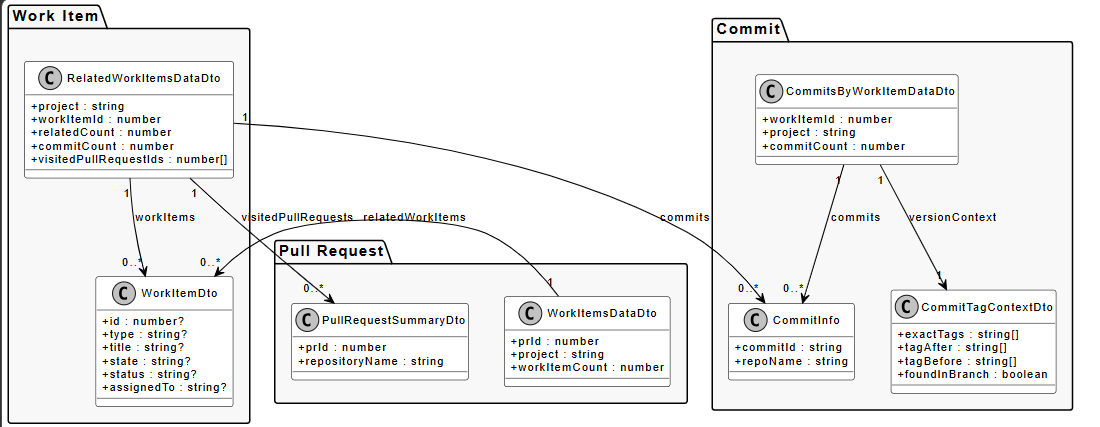
\includegraphics[width=1\linewidth]{img/archi/workitems_pr_commit_class_diag.png}
    \caption{Backend class diagram for the work item, pull request, and commit modules}
    \label{fig:backend-workitem-pr-commit-class-diagram}
\end{figure}

\begin{figure}[H]
    \centering
    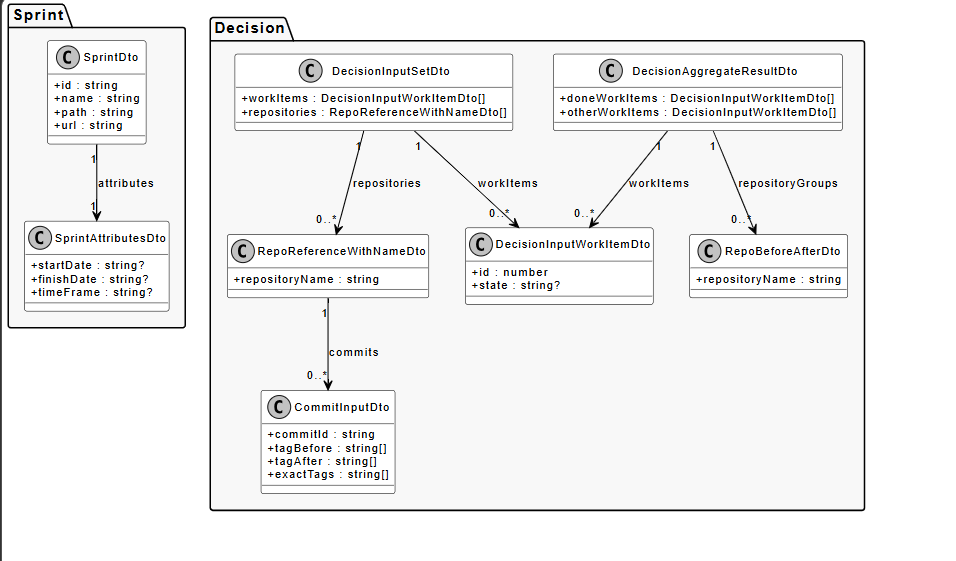
\includegraphics[width=1\linewidth]{img/archi/sprint_decision_class_diag.png}
    \caption{Backend class diagram for the sprint and decision modules}
    \label{fig:backend-sprint-decision-class-diagram}
\end{figure}

\subsection{API Contract Design}

The backend exposes a set of RESTful endpoints that support both single and
batch traceability analysis with a consistent response model.

\begin{description}
  \item[Single related endpoint]
  \texttt{/workitem/:id/related}

  Returns a traceability graph centered on a single root work item.

  \item[Batch related endpoint]
  \texttt{/workitem/related}

  Returns an aggregated, deduplicated graph for multiple root items.

  \item[Tasks stream endpoint]
  \texttt{/workitem/tasks/stream}

  Streams processing results progressively using Server-Sent Events (SSE).

  \item[PR-to-work-items endpoint]
  \texttt{/pullrequests/:prId/workitems}

  Retrieves work items linked to a given pull request.

  \item[Sprint listing endpoint]
  \texttt{/sprint?project=...}

  Returns the iterations available for a project.

  \item[Sprint work-items endpoint]
  \texttt{/sprint/:sprintId/work-items?project=...}

  Returns work items for a given sprint and supports lazy loading in the UI.

  \item[Commit tag batch endpoint]
  \texttt{/commits/tags/batch}

  Enriches commit references with repository tag metadata.

  \item[LLM commit review endpoint]
  \texttt{/commits/hf/review}

  Generates an AI-assisted review for a selected commit using repository and
  commit context.
\end{description}

The DTO strategy prioritizes:
\begin{itemize}
  \item stable response contracts between the backend and its consumers;
  \item best-effort metadata enrichment (e.g., repository names for visited PRs);
  \item a clear separation between operational traceability contracts and
  optional AI-generated review payloads;
  \item explicit counters and trace metadata for UI sorting and interpretation.
\end{itemize}

\subsection{Implementation Characteristics}

\begin{itemize}
  \item graph traversal with visited-state tracking to prevent cycles;
  \item request-scoped caching and batched retrieval to reduce external API load;
  \item normalization of external payloads before propagation between services;
  \item structured logging to support diagnostics and operational monitoring.
\end{itemize}

\subsection{Sequence and Processing Flows}

Backend processing is built around orchestration pipelines where each service
builds on the output of the previous stage.

\begin{itemize}
  \item \textbf{Single-root flow:} resolve the root work item, traverse related
  nodes, enrich pull requests and commits, return a normalized graph.
  \item \textbf{Batch flow:} run multi-root traversal with deduplication and
  consolidated counters.
  \item \textbf{Sprint exploration flow:} load project sprints, lazily fetch
  sprint work items, then forward selected items to the batch flow.
  \item \textbf{Commit tag flow:} resolve tag context in batch, grouped by
  repository, using a latest-tag strategy.
  \item \textbf{LLM review flow:} collect commit metadata and relevant file
  snapshots, augment the prompt with repository guidance, invoke the model,
  and return the generated review to the decision UI.
\end{itemize}

\begin{figure}[H]
  \noindent\makebox[\textwidth][c]{%
  
\includegraphics[width=\paperwidth,height=0.94\textheight,keepaspectratio]{"img/archi/single-root related-work-item processing.png"}
  }
  \caption{Sequence diagram for single-root related work-item processing}
  \label{fig:work-item-related-sequence}
\end{figure}

\begin{figure}[H]
\noindent\makebox[\textwidth][c]{%
  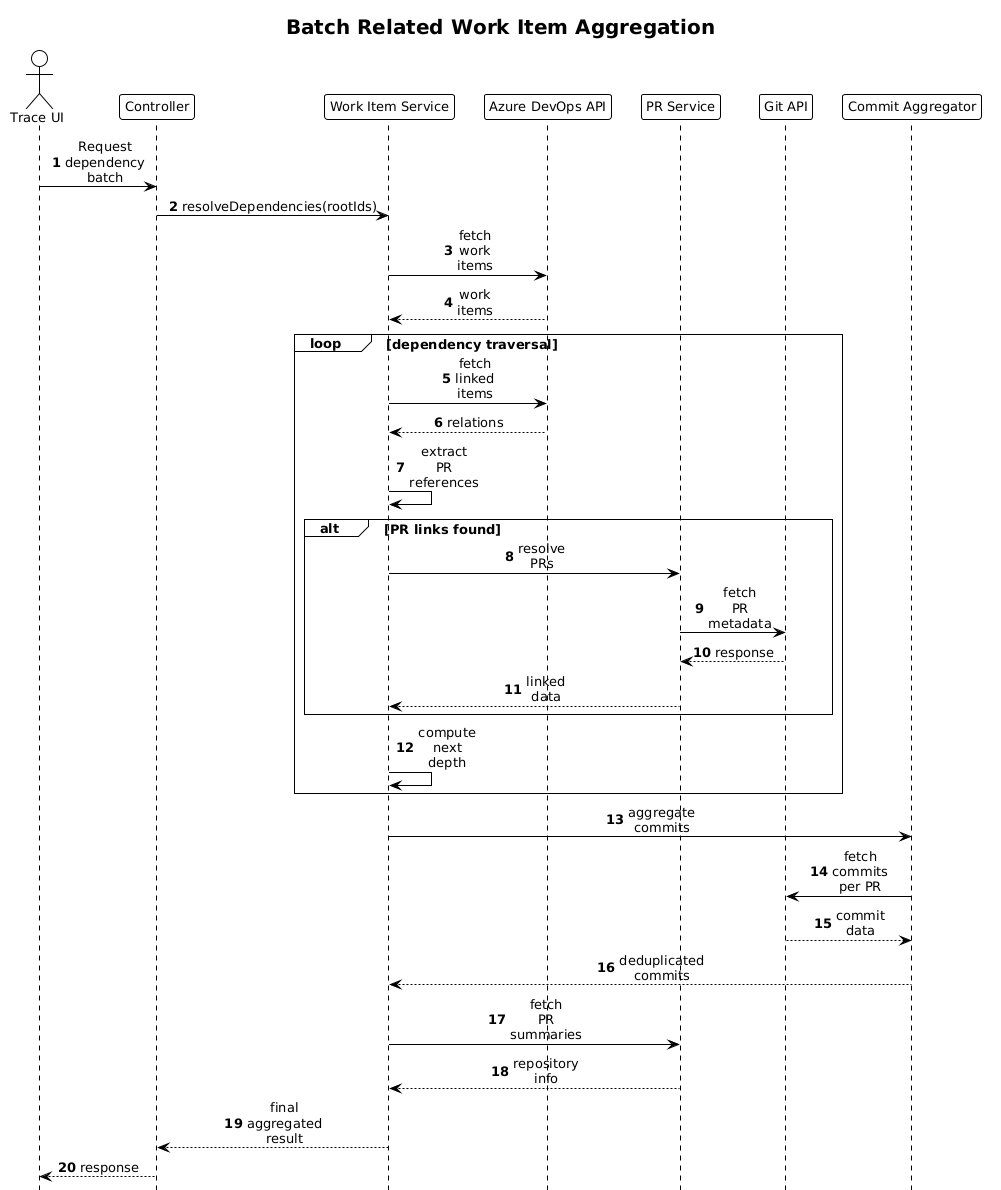
\includegraphics[width=\paperwidth,height=0.94\textheight,keepaspectratio]{img/archi/BatchRelatedWorkItem.png}
}
  \caption{Sequence diagram for batch related work-item aggregation}
  \label{fig:work-item-batch-sequence}
\end{figure}

% ──────────────────────────────────────────────────────────────────────────────
\section{UI Implementation}

\subsection{UI Architecture and Main Surfaces}

The UI layer is the main entry point to the traceability system. It is
organized around route-driven views that map to the key analysis scenarios,
with a shared state and API integration layer handling requests, progressive
loading, and result display.

\begin{itemize}
  \item \textbf{RelatedWorkItemTrace:} single-root analysis screen for
  exploring one work item and its related artifacts.
  \item \textbf{BatchWorkItemTrace:} selection and loading screen for
  progressively collecting candidate work items through SSE streaming.
  \item \textbf{SprintWorkItemsView:} planning-oriented screen for loading
  sprints, lazily fetching their work items, and preparing cross-sprint
  selections.
  \item \textbf{BatchRelatedWorkItemTrace:} aggregated result screen showing
  the consolidated output of multi-root analysis with commit and repository
  context.
  \item \textbf{DecisionDashboard:} decision and promotion screen extended
  with commit-level LLM review actions.
\end{itemize}

\begin{figure}[H]
\noindent\makebox[\textwidth][c]{%
  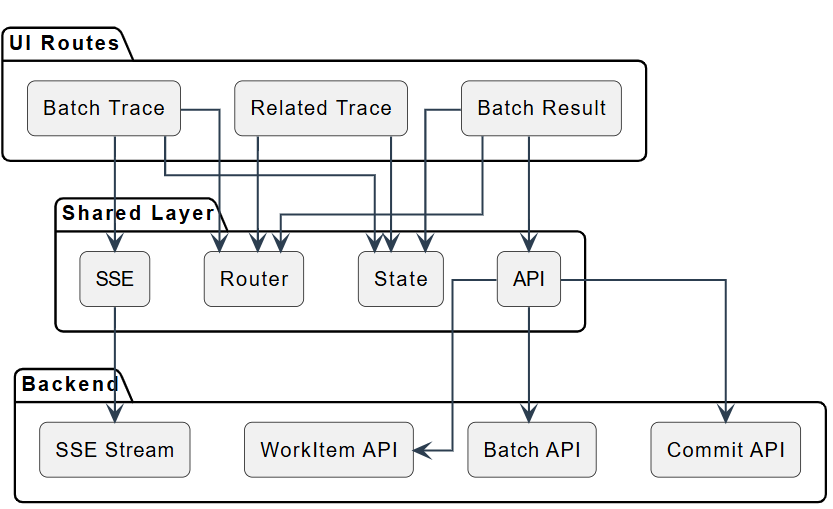
\includegraphics[width=\paperwidth]{img/figures/uiroutes.png}
}
  \caption{UI route and component architecture for traceability workflows}
  \label{fig:ui-route-component-diagram}
\end{figure}

\subsection{UI Data Flow and Backend Integration}

The UI communicates with the backend through a dedicated trace API layer and
maps backend contracts to typed frontend models.

\begin{itemize}
  \item Single analysis uses \texttt{/workitem/:id/related}.
  \item Batch task loading consumes \texttt{/workitem/tasks/stream} via SSE.
  \item Sprint exploration calls \texttt{/sprint} and
  \texttt{/sprint/:sprintId/work-items} with lazy retrieval per expanded sprint.
  \item Batch result enrichment uses \texttt{/commits/tags/batch} grouped by
  repository.
  \item Commit-level review actions call \texttt{/commits/review} from the
  decision dashboard when the operator requests an AI-generated assessment.
  \item Authentication failures trigger a controlled redirect when the backend
  returns an unauthorized response.
\end{itemize}

\begin{figure}[H]
  \noindent\makebox[\textwidth][c]{%
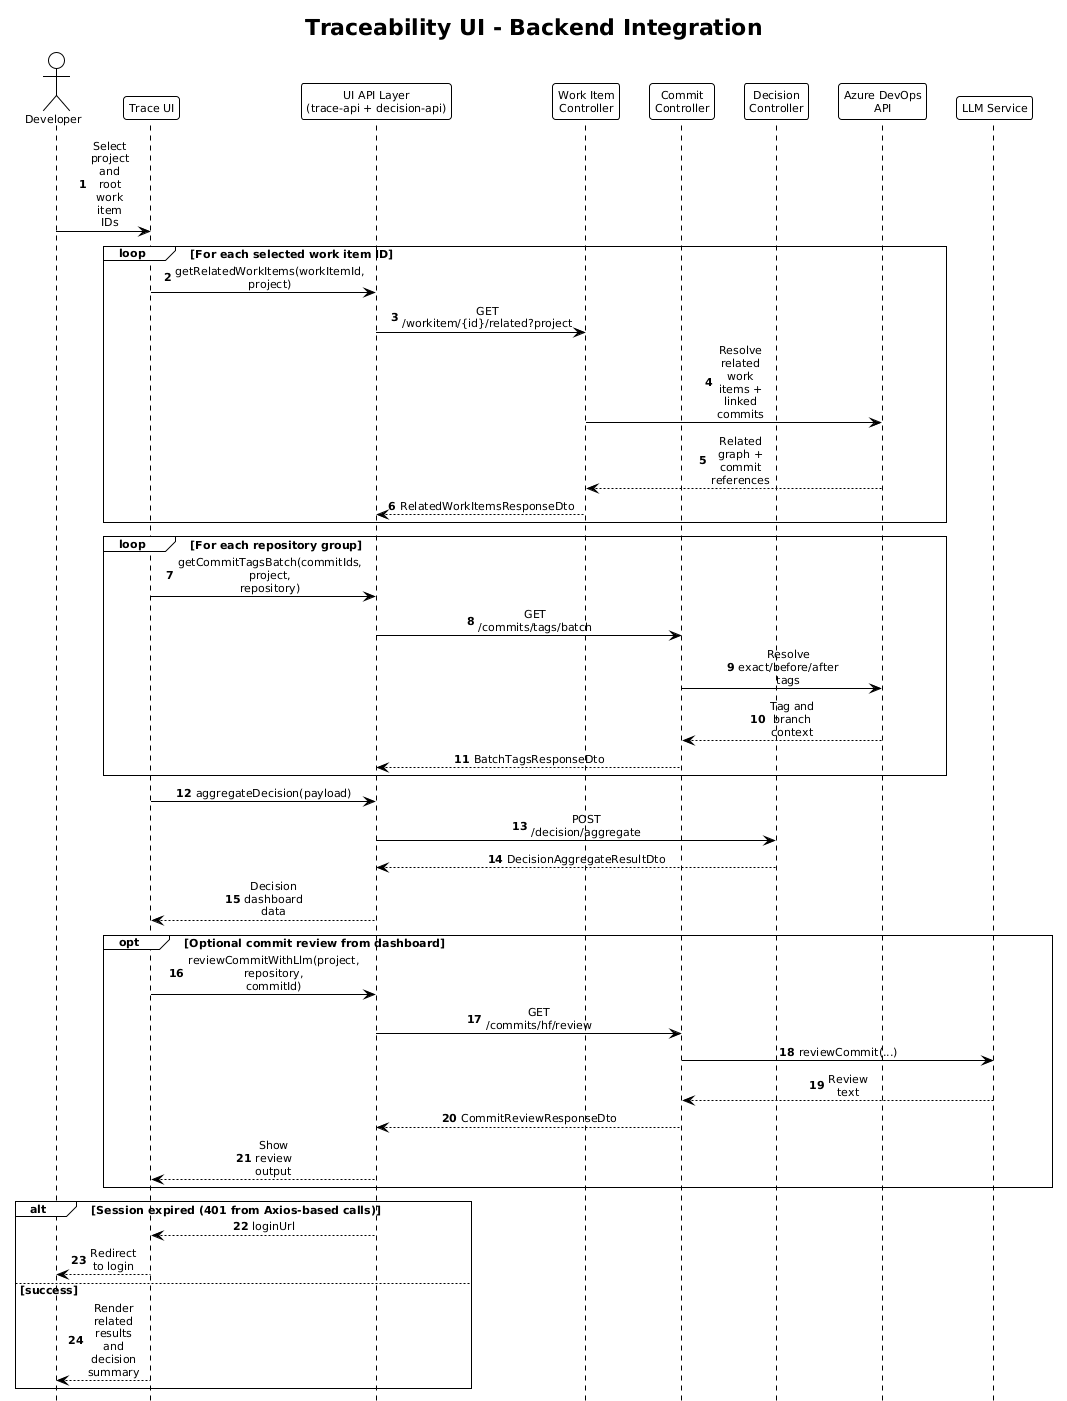
\includegraphics[width=\paperwidth,height=0.90\textheight,keepaspectratio]{img/archi/backend_uiflow.png}}
\caption{Sequence diagram for UI and backend integration in trace workflows}
\label{fig:ui-backend-integration-sequence}
\end{figure}


\subsection{UI Operational Considerations}

\begin{itemize}
  \item progressive loading to keep batch interactions responsive;
  \item consistent result ordering based on traceability counters;
  \item graceful rendering when enrichment metadata is partially unavailable.
\end{itemize}

\subsection{Screens and UI Walkthrough}

\subsubsection{Batching Work Items}

This screen is used to select multiple work items for batch processing and kick
off a batched traceability run. Selection is flexible --- single items, multiple,
or all at once --- and run progress is shown progressively using Server-Sent
Events (SSE). The screen includes quick filters and tools for prioritizing
candidates before downstream aggregation.

\begin{figure}[htbp]
\noindent\makebox[\textwidth][c]{%
  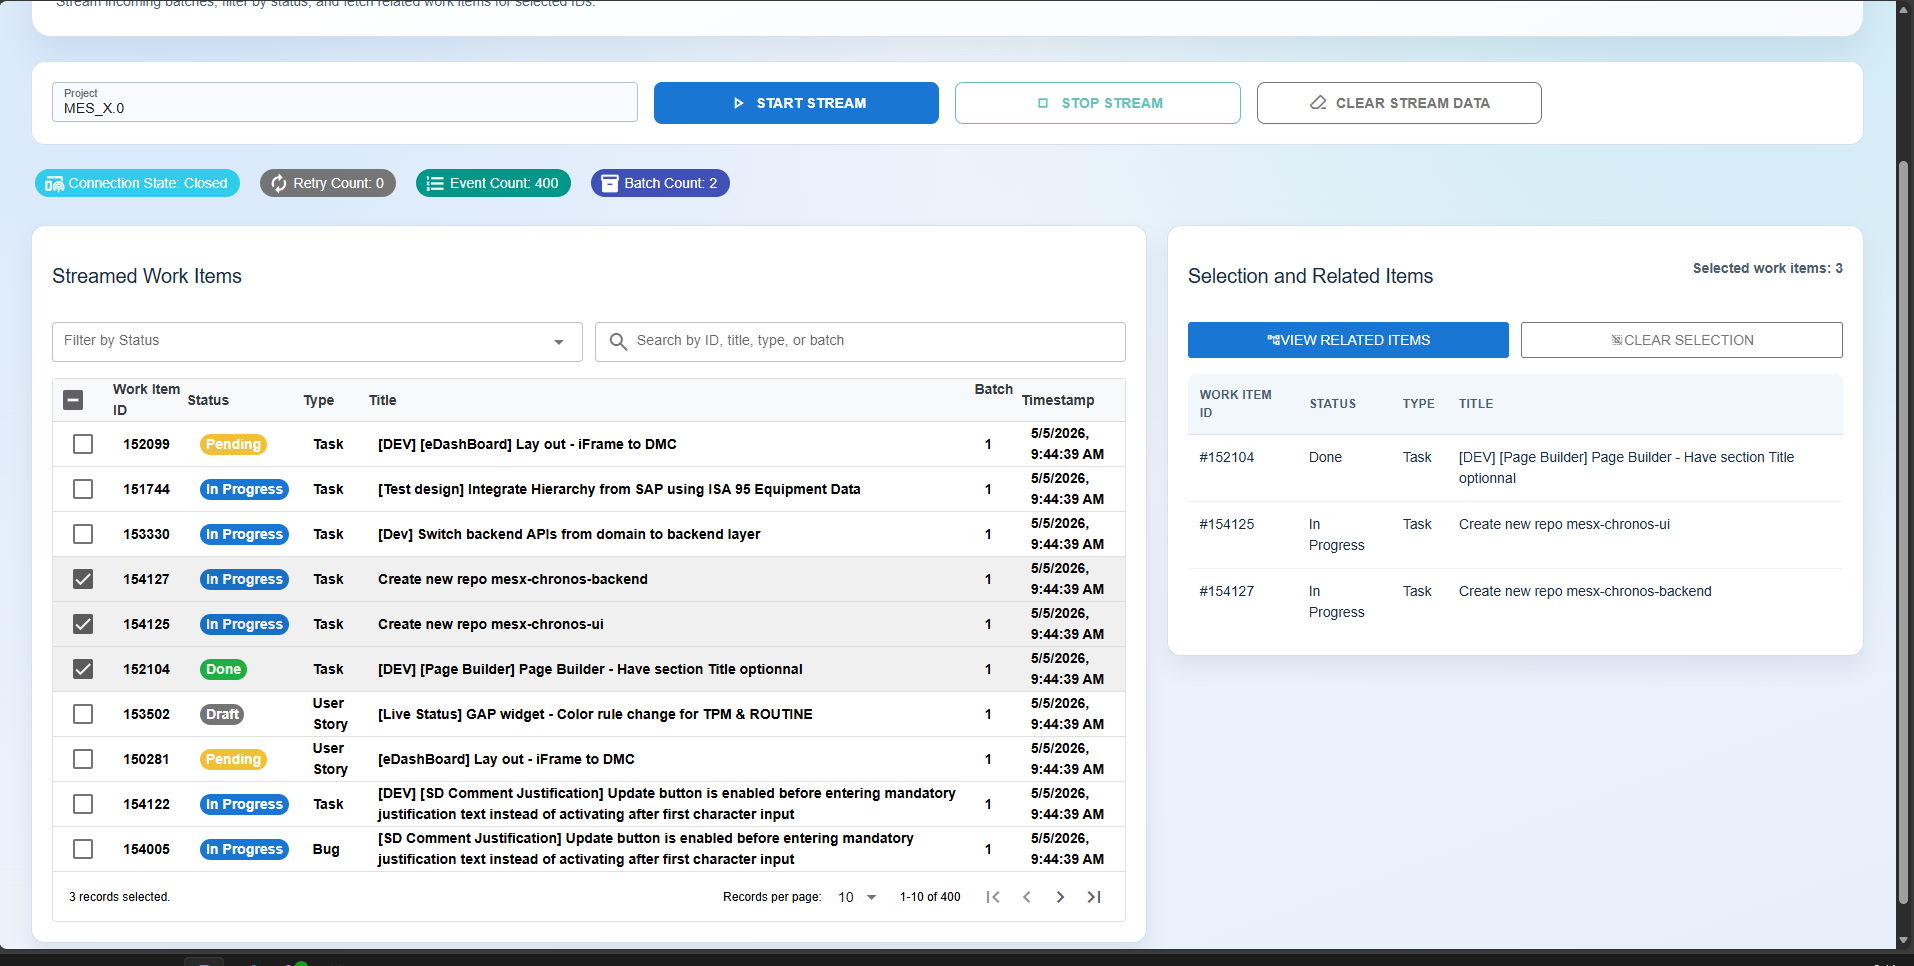
\includegraphics[width=\paperwidth]{img/figures/ui-batch-task-screen.png}
}
  \caption{Batching Work Items -- selection and SSE-driven progress}
  \label{fig:batching-wi}
\end{figure}

\subsubsection{Get Related}

The "Get Related" flow has two complementary screens:

\begin{figure}[htbp]
\noindent\makebox[\textwidth][c]{%
  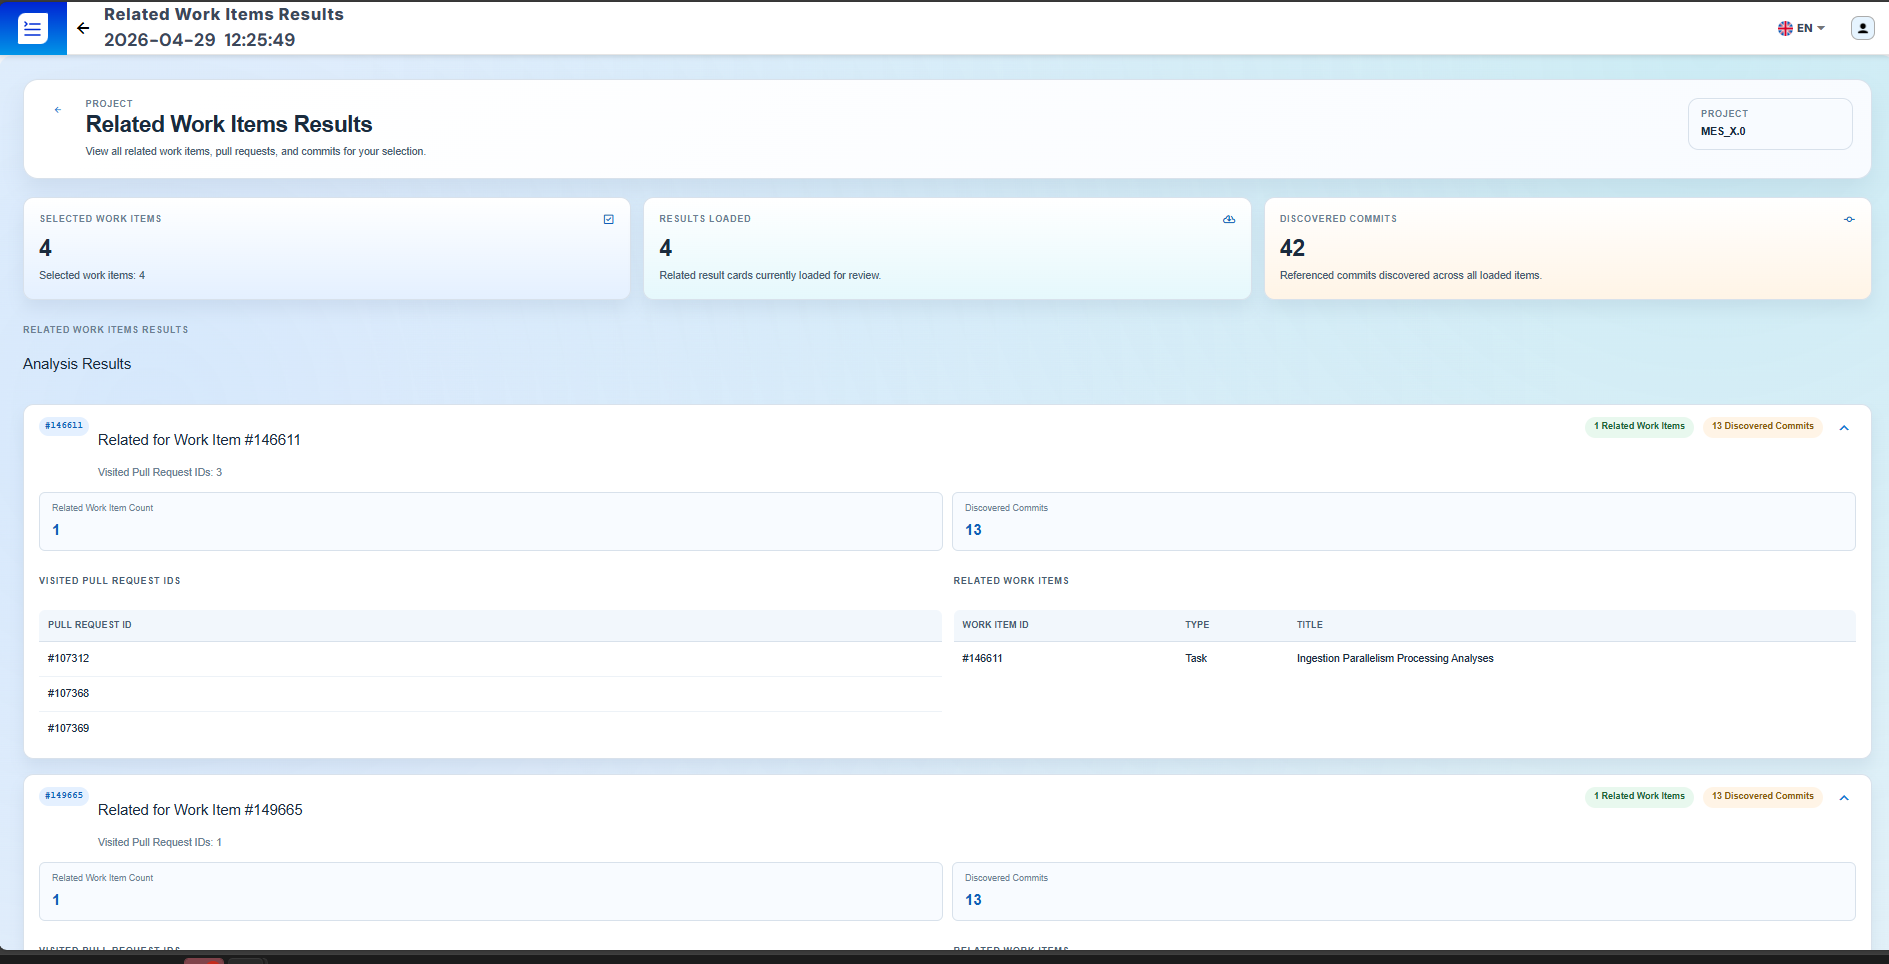
\includegraphics[width=\paperwidth]{img/figures/related-workitem1.png}
}
  \caption{Related Work Item -- single-root traceability graph view}
  \label{fig:related-workitem}
\end{figure}

The Related Work Item view shows a single root work item and its connected
graph (pull requests, commits, branches, tags). Nodes can be expanded and
inspected, and the operator can drill down to commit or PR level.

\begin{figure}[htbp]
\noindent\makebox[\textwidth][c]{%
  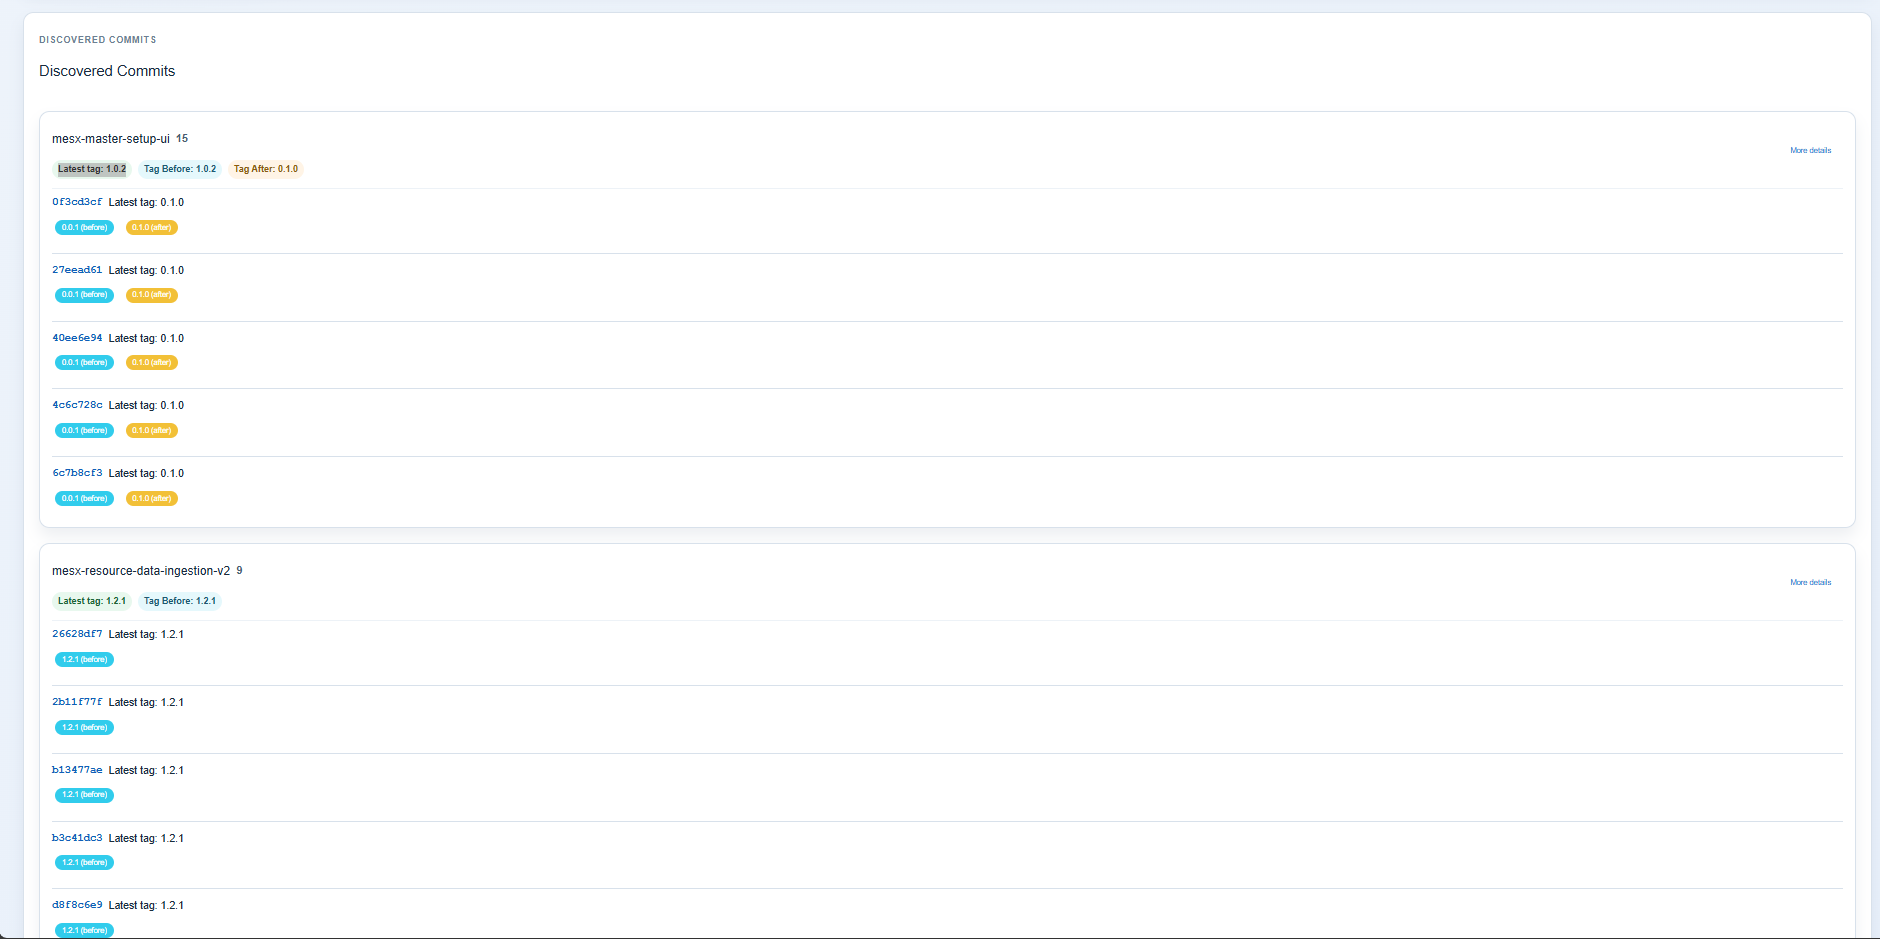
\includegraphics[width=\paperwidth]{img/figures/discovered-commits.png}
}
  \caption{Discovered Commits -- commits found during traversal}
  \label{fig:discovered-commits}
\end{figure}

The Discovered Commits screen lists commits found during traversal along with
contextual metadata: branch, tags, and associated work items. This view is
useful for verifying commit-to-work-item linkage and checking tag context
before any automated decisions are made.

\subsubsection{Sprint Work Items}

The Sprint Work Items screen provides a planning-driven entry point to the
traceability workflow. Rather than starting from manually entered identifiers,
the operator loads the sprint list for a project and expands individual sprint
cards to lazily fetch their work items. Selected items are kept across loaded
sprints and can be forwarded directly to the batch analysis flow.

\subsubsection{Decision}

The Decision section provides summarized outputs to guide promotion actions.
It contains two key screens:

\begin{figure}[htbp]
\noindent\makebox[\textwidth][c]{%
  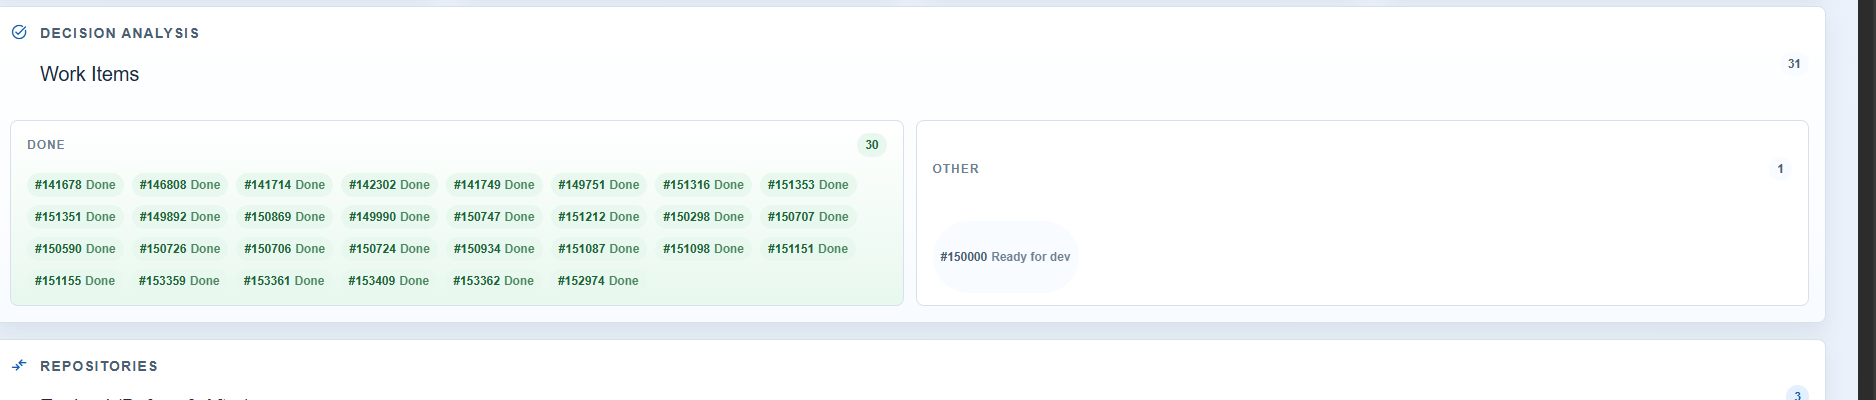
\includegraphics[width=\paperwidth]{img/figures/decision-wi-state.png}
}
  \caption{Decision -- work items grouped by state (Done vs. Other)}
  \label{fig:decision-wi-state}
\end{figure}

The first Decision view groups work items by state (for example, \texttt{Done}
vs \texttt{Other}) so operators can quickly see which items are ready for
promotion and which still need attention.

\begin{figure}[htbp]
\noindent\makebox[\textwidth][c]{%
  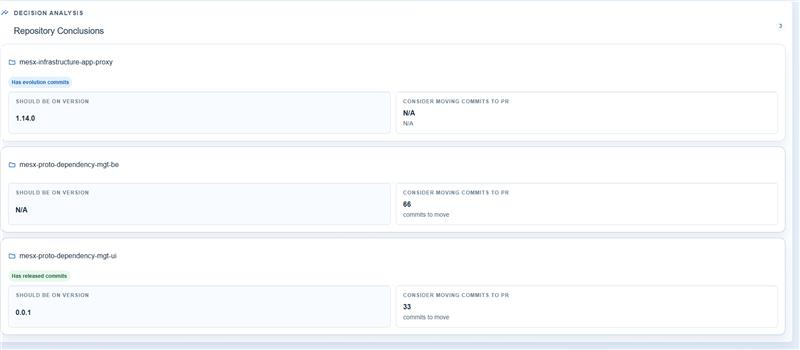
\includegraphics[width=\paperwidth]{img/figures/decision-repo-tags.jpg}
}
  \caption{Decision -- repository view with expected tags for promotion}
  \label{fig:decision-repo-tags}
\end{figure}

The repository/tags screen shows, per repository, the commits and expected tags
(before/after/exact) that the system identified. From here, an operator can
select a candidate work item and trigger a promotion workflow (for example:
move a work item to production) after reviewing tag context. The same screen
also exposes an LLM review action on eligible commits, allowing the operator
to request an AI-generated assessment before making a final decision.

% ──────────────────────────────────────────────────────────────────────────────
\section{Docker Orchestration and Deployment}

\subsection{Service Orchestration Model}

The backend runtime is packaged as an isolated service with clearly defined
integration boundaries.

\begin{itemize}
  \item The backend container exposes REST/SSE APIs on the configured runtime port.
  \item Runtime configuration and secrets are injected through environment
  variables and externalized config files.
  \item The backend accesses Azure DevOps Work Item and Git APIs over HTTPS.
\end{itemize}

\subsection{Operational Dependencies}

\begin{itemize}
  \item CI/CD pipeline for image build and deployment validation.
  \item Optional caching layer through internal cache services.
  \item Secrets and environment values injected at runtime.
\end{itemize}

\subsection{Deployment Objectives}

\begin{itemize}
  \item reproducible execution locally and in CI;
  \item independent versioning and rollout of backend artifacts;
  \item reduced deployment risk through clear component ownership.
\end{itemize}

% ──────────────────────────────────────────────────────────────────────────────
\section{Quality, Security, and Operational Considerations}

\subsection{Testing and Validation}

Validation was carried out at multiple levels to ensure the delivered solution
matched the requirements defined earlier in this report.

\begin{itemize}
  \item Backend unit tests covered controller and service behavior, especially
  work item traversal, commit resolution, and DTO mapping.
  \item End-to-end tests validated the main API flows and confirmed the
  frontend correctly consumed the backend contracts.
  \item Frontend quality checks combined linting, style validation, and manual
  testing of the main traceability views and the decision dashboard.
  \item Cross-layer checks ensured that streaming behavior, repository grouping,
  and decision outputs remained consistent from backend to UI.
\end{itemize}

\subsection{Developed Tests}

The test effort focused on validating the most critical traceability services
and API contracts used by the UI.

\begin{itemize}
  \item \textbf{Backend unit tests (Jest):} implemented for the Work Item,
  Commit, and Sprint modules, including controller and service-level behavior.
  \item \textbf{Backend utility tests:} added for tag-selection logic used by
  repository context enrichment.
  \item \textbf{Backend API end-to-end test:} implemented under the
  \texttt{test/} suite to validate core HTTP integration behavior.
  \item \textbf{Frontend validation:} performed through linting, static checks,
  and manual scenario-based verification of key traceability screens.
\end{itemize}

\textbf{Quality controls:}
\begin{itemize}
  \item controller-level input validation and typed DTO contracts;
  \item service-level tests for traversal, tag selection, and data normalization;
  \item regression-focused tests for traversal and normalization behavior.
\end{itemize}

\textbf{Security and runtime controls:}
\begin{itemize}
  \item secure communication for all backend integrations;
  \item managed access to Azure DevOps external APIs;
  \item structured logging to support incident analysis and diagnostics.
\end{itemize}

% ──────────────────────────────────────────────────────────────────────────────
\section{AI-assisted Development and Review}

AI-assisted tools were used throughout the project to support both backend and
frontend work. The goal was not to replace engineering decisions, but to speed
up repetitive tasks, improve review coverage, and encode project-specific
conventions.

The application also ships an operational LLM capability within the backend
itself. The Commit module delegates review requests to a dedicated LLM module
that builds prompts from Azure DevOps commit metadata, selects a small set of
relevant changed files, injects repository instructions and skill guidance, and
calls an external model to produce a structured review. This review is then
surfaced in the decision dashboard, so release analysis can be complemented by
code-level observations when needed.

Both repositories keep their automation artifacts inside the codebase. On the
backend, the \texttt{.github/agents/} directory defines dedicated roles such as
architect, implementer, reviewer, and QA agent. On the frontend,
\texttt{.github/agents/}, \texttt{.github/instructions/}, and
\texttt{.github/skills/} capture UI guidelines, review rules, and reusable
workflows for Vue, Quasar, styling, and quality checks. Keeping these files
versioned alongside the source code makes the automation explicit, reviewable,
and reproducible.

In practice, these agents assisted with code drafting, refactoring, test
scaffolding, documentation, and architecture reviews. The instruction files
helped enforce conventions such as typed contracts, logging discipline,
component structure, localization, and style consistency. On the frontend they
reinforced guardrails around Vue Composition API usage, token-based styling,
and UI quality. On the backend they kept DTO usage, controller-service
separation, and observability patterns consistent across the codebase.

All AI-generated suggestions went through human review. Proposed changes were
treated as drafts and validated through linting, SonarQube policies, tests, and
direct developer inspection before being merged. This made AI tools genuinely
useful across both development and runtime review support, while keeping
accountability, technical rigor, and architectural coherence firmly in human
hands.

% ──────────────────────────────────────────────────────────────────────────────
\section*{Conclusion}

The implementation produced a modular traceability platform combining a
graph-oriented backend, an operational frontend, and a deployment-ready runtime
configuration. The result replaces a manual, fragmented analysis process with a
structured workflow that is faster, easier to interpret, and better suited to
release preparation.

By combining layered design, iterative development, thorough validation, and
careful integration with Azure DevOps, the project built a maintainable
foundation for dependency analysis, release decision support, and future
expansion of the traceability scope.

\addcontentsline{toc}{section}{Conclusion}